\documentclass[10.5pt,a4paper]{article}
\usepackage[margin=1.9cm,top=2.1cm,bottom=1.9cm]{geometry}
\usepackage[T1]{fontenc}
\usepackage{lmodern}
\usepackage{amsmath,amssymb}
\usepackage{enumitem}
\usepackage{booktabs,array}
\usepackage{xcolor}
\usepackage{fancyhdr}
\usepackage[most]{tcolorbox}
\usepackage{tikz}
\usetikzlibrary{automata,positioning,arrows.meta,calc,trees}
\usepackage[hidelinks,pdftitle={CSE 211 Term Final 2024-25 Solutions}]{hyperref}

\definecolor{navy}{HTML}{1F3864}
\definecolor{qbg}{HTML}{F6F6F6}
\definecolor{exbg}{HTML}{F4FAF4}
\definecolor{exborder}{HTML}{2E7D32}
\definecolor{trapborder}{HTML}{C62828}

\setlist{itemsep=1pt,topsep=3pt,parsep=0pt,leftmargin=1.5em}
\setlength{\parindent}{0pt}
\setlength{\parskip}{4pt}
\renewcommand{\arraystretch}{1.15}

\pagestyle{fancy}
\fancyhf{}
\lhead{\small\color{gray}CSE 211 --- Term final 2024-25 (10/11/2026): solutions}
\rhead{\small\color{gray}\leftmark}
\cfoot{\small\color{gray}\thepage}
\renewcommand{\headrulewidth}{0.3pt}

\newtcolorbox{qa}[2]{breakable,enhanced,colback=qbg,colbacklower=exbg,colframe=exborder,boxrule=0.5pt,leftrule=3pt,arc=1pt,
  left=7pt,right=7pt,top=4pt,bottom=4pt,title={Question #1 \hfill (#2)},fonttitle=\bfseries\small,coltitle=white,
  colbacktitle=exborder,segmentation style={solid,exborder,line width=0.4pt},before skip=9pt,fontupper=\itshape}
\newcommand{\ansh}[1]{\textbf{\color{exborder}#1}\ }

\tikzset{every state/.style={minimum size=0.8cm,inner sep=1pt,font=\small},
  >={Stealth[length=2mm]},auto,node distance=2.1cm,every edge/.append style={font=\small}}

\newcommand{\eps}{\varepsilon}
\newcommand{\NP}{\mathrm{NP}}
\renewcommand{\P}{\mathrm{P}}
\newcommand{\PS}{\mathrm{PSPACE}}
\newcommand{\NPS}{\mathrm{NPSPACE}}
\newcommand{\Ld}{L_d}
\newcommand{\Lu}{L_u}

\begin{document}

\begin{center}
{\Large\bfseries\color{navy} CSE 211 --- Theory of Computation}\\[2pt]
{\large L-2/T-II B.Sc.\ Engineering Examinations 2024-2025 (held 10/11/2026): exam-ready solutions}\\[2pt]
{\small Section A: answer any seven of Questions 1--9 \quad$\cdot$\quad Section B: Question 10 compulsory, any two of 11--13}
\end{center}

\begin{tcolorbox}[colback=white,colframe=navy,boxrule=0.4pt,arc=1pt,left=6pt,right=6pt,top=3pt,bottom=3pt]
All thirteen questions are answered. Each grey box is the question as printed; below the line is the answer as it would be written in the
script. Section A follows Atif Sir's notation (Hopcroft--Motwani--Ullman); Section B follows Hakim Sir's (Sipser).\\[2pt]
\textbf{Checked by program} (\texttt{\_build/verify\_2425\_final.py}, all pass): the PDA of Q1 (all strings up to length 10), the PDAs of Q2(a)
and Q2(b) against the grammar (up to length 5), the TM of Q4 (every input of length 1--7), the DFA of Q10(b) (up to length 12, and its 8 states
are pairwise distinguishable), the grammars of Q10(c) and Q12(c), the NFA of Q11(b), and the NFA of Q13(c) against $(ab^*c\cup ac)^*$.
The proofs and explanations are standard textbook arguments following the course slides.
\end{tcolorbox}

\tableofcontents

% ======================================================================= SECTION A
\clearpage
\section*{Section A}\addcontentsline{toc}{section}{Section A}

\section{Question 1 --- PDA for $\{a^ib^jc^k\mid j=i+k\}$}\markboth{Q1 PDA}{}
\begin{qa}{1}{15 marks}
Design a pushdown automaton (PDA) that recognizes the following language by final state: $L=\{a^ib^jc^k\mid j=i+k\}$. Draw its transition diagram.
\tcblower
\ansh{Idea.} $j=i+k$ means the $b$'s split into a first group matched with the $a$'s and a second group matched with the $c$'s:
$a^i\,b^i\,b^k\,c^k$. So: push an $X$ for every $a$; for every $b$ pop an $X$ while there is one; once $Z_0$ is back on top, push a $Y$ for
every further $b$; pop a $Y$ for every $c$. Accept (move to the final state) when $Z_0$ is on top again and the input is finished.\\
\ansh{Stack symbols.} $X$ = an $a$ still waiting for its $b$; $Y$ = a $b$ still waiting for its $c$; $Z_0$ = bottom (everything matched).\\
\ansh{States.} $q_0$: reading $a$'s; $q_1$: reading $b$'s; $q_2$: reading $c$'s; $q_f$: accepting.
\[P=(\{q_0,q_1,q_2,q_f\},\ \{a,b,c\},\ \{X,Y,Z_0\},\ \delta,\ q_0,\ Z_0,\ \{q_f\})\]
\begin{center}\small
\begin{tabular}{@{}lll@{}}
\toprule
from & transitions & meaning\\\midrule
$q_0$ & $\delta(q_0,a,Z_0)=\{(q_0,XZ_0)\}$,\ $\delta(q_0,a,X)=\{(q_0,XX)\}$ & push one $X$ per $a$\\
$q_0$ & $\delta(q_0,b,X)=\{(q_1,\eps)\}$,\ $\delta(q_0,b,Z_0)=\{(q_1,YZ_0)\}$ & first $b$ (matches an $a$, or $i=0$)\\
$q_1$ & $\delta(q_1,b,X)=\{(q_1,\eps)\}$ & $b$ matched with an $a$\\
$q_1$ & $\delta(q_1,b,Z_0)=\{(q_1,YZ_0)\}$,\ $\delta(q_1,b,Y)=\{(q_1,YY)\}$ & extra $b$'s, to be matched with $c$'s\\
$q_1$ & $\delta(q_1,c,Y)=\{(q_2,\eps)\}$;\quad $\delta(q_2,c,Y)=\{(q_2,\eps)\}$ & $c$ matched with a $b$\\
$q_0,q_1,q_2$ & $\delta(q,\eps,Z_0)=\{(q_f,Z_0)\}$ & all matched: accept\\\bottomrule
\end{tabular}
\end{center}
\begin{center}
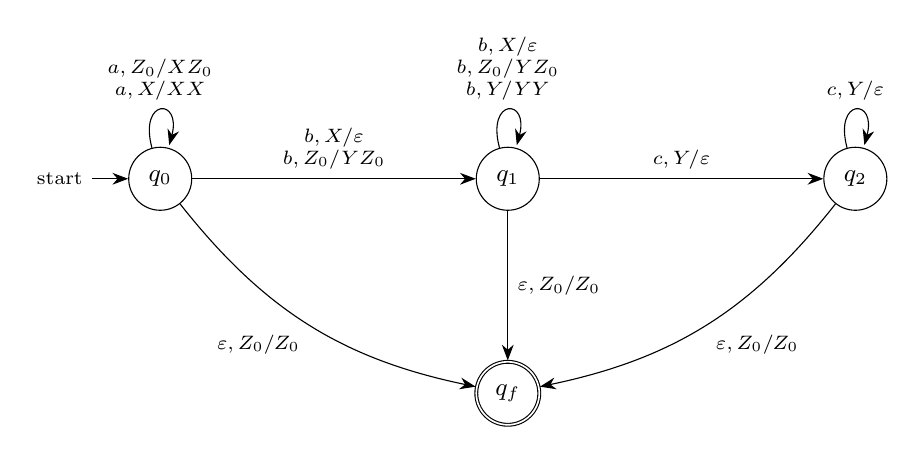
\begin{tikzpicture}[node distance=3.6cm,every edge/.append style={font=\scriptsize}]
\node[state,initial] (0) {$q_0$};
\node[state,right=of 0] (1) {$q_1$};
\node[state,right=of 1] (2) {$q_2$};
\node[state,accepting,below=1.9cm of 1] (f) {$q_f$};
\path[->] (0) edge[loop above] node[align=center] {$a,Z_0/XZ_0$\\$a,X/XX$} ()
 (0) edge node[align=center] {$b,X/\eps$\\$b,Z_0/YZ_0$} (1)
 (1) edge[loop above] node[align=center] {$b,X/\eps$\\$b,Z_0/YZ_0$\\$b,Y/YY$} ()
 (1) edge node {$c,Y/\eps$} (2)
 (2) edge[loop above] node {$c,Y/\eps$} ()
 (0) edge[bend right=20] node[swap] {$\eps,Z_0/Z_0$} (f)
 (1) edge node {$\eps,Z_0/Z_0$} (f)
 (2) edge[bend left=20] node {$\eps,Z_0/Z_0$} (f);
\end{tikzpicture}
\end{center}
\ansh{Why it works.} An $X$ can only be above $Z_0$ while $a$'s are unmatched, and a $Y$ only after all $X$'s are gone, so $b$'s first cancel
$a$'s and then wait for $c$'s. Reading $c$ with $X$ on top ($j<i$), or finishing with $Y$ or $X$ on the stack, leaves no way to $q_f$.\\
\ansh{Accepted: $abbbcc$} ($i=1$, $j=3$, $k=2$):
$(q_0,abbbcc,Z_0)\vdash(q_0,bbbcc,XZ_0)\vdash(q_1,bbcc,Z_0)\vdash(q_1,bcc,YZ_0)\vdash(q_1,cc,YYZ_0)\vdash(q_2,c,YZ_0)\vdash(q_2,\eps,Z_0)\vdash(q_f,\eps,Z_0)$
--- accept.\\
\ansh{Rejected: $abbbc$} ($j=3\ne2$): $\dots\vdash(q_1,c,YYZ_0)\vdash(q_2,\eps,YZ_0)$; $Y$ is on top, so the $\eps,Z_0$ move is impossible --- reject.
\end{qa}

\section{Question 2 --- CFG to PDA, empty stack to final state}\markboth{Q2 CFG to PDA}{}
\begin{qa}{2(a)}{8 marks}
Design a PDA that uses acceptance by empty stack to recognize the language generated by the CFG (start symbol $E$):
$E\to E+T\mid T$,\ $T\to T\times F\mid F$,\ $F\to(E)\mid I$,\ $I\to a\mid b$.
\tcblower
\ansh{Construction (CFG $\to$ PDA).} The PDA simulates leftmost derivations with one state. When a variable is on top, it replaces it by the
body of one of its productions (nondeterministic choice); when a terminal is on top, it must match the next input symbol.
\[P_N=(\{q\},\ \{a,b,+,\times,(,)\},\ \{E,T,F,I,a,b,+,\times,(,)\},\ \delta,\ q,\ E)\]
\begin{enumerate}
\item $\delta(q,\eps,E)=\{(q,E+T),\ (q,T)\}$
\item $\delta(q,\eps,T)=\{(q,T\times F),\ (q,F)\}$
\item $\delta(q,\eps,F)=\{(q,(E)),\ (q,I)\}$
\item $\delta(q,\eps,I)=\{(q,a),\ (q,b)\}$
\item $\delta(q,t,t)=\{(q,\eps)\}$ for every terminal $t\in\{a,b,+,\times,(,)\}$.
\end{enumerate}
\begin{center}
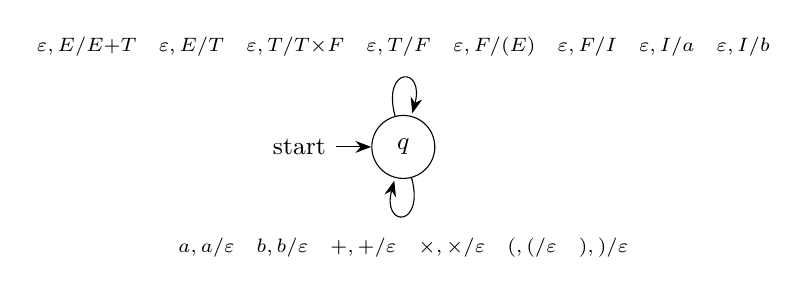
\begin{tikzpicture}
\node[state,initial] (q) {$q$};
\path[->] (q) edge[loop above] () (q) edge[loop below] ();
\node[above=0.62cm of q,font=\scriptsize] {$\eps,E/E{+}T\quad \eps,E/T\quad \eps,T/T{\times}F\quad \eps,T/F\quad \eps,F/\mathtt{(}E\mathtt{)}\quad \eps,F/I\quad \eps,I/a\quad \eps,I/b$};
\node[below=0.62cm of q,font=\scriptsize] {$a,a/\eps\quad b,b/\eps\quad {+},{+}/\eps\quad {\times},{\times}/\eps\quad \mathtt{(},\mathtt{(}/\eps\quad \mathtt{)},\mathtt{)}/\eps$};
\end{tikzpicture}
\end{center}
\ansh{Trace on $a+b\times a$} (follows the leftmost derivation $E\Rightarrow E+T\Rightarrow T+T\Rightarrow F+T\Rightarrow I+T\Rightarrow a+T\Rightarrow
a+T\times F\Rightarrow\dots\Rightarrow a+b\times a$):
\[\begin{aligned}
&(q,a{+}b{\times}a,E)\vdash(q,a{+}b{\times}a,E{+}T)\vdash(q,a{+}b{\times}a,T{+}T)\vdash(q,a{+}b{\times}a,F{+}T)\vdash(q,a{+}b{\times}a,I{+}T)\\
&\vdash(q,a{+}b{\times}a,a{+}T)\vdash(q,{+}b{\times}a,{+}T)\vdash(q,b{\times}a,T)\vdash(q,b{\times}a,T{\times}F)\vdash(q,b{\times}a,F{\times}F)\\
&\vdash(q,b{\times}a,I{\times}F)\vdash(q,b{\times}a,b{\times}F)\vdash(q,{\times}a,{\times}F)\vdash(q,a,F)\vdash(q,a,I)\vdash(q,a,a)\vdash(q,\eps,\eps)\\
&\text{--- stack empty, accept.}
\end{aligned}\]
At every point, (input read) followed by (stack contents) is a leftmost sentential form, so $N(P_N)=L(G)$.
\end{qa}

\begin{qa}{2(b)}{7 marks}
Now convert the PDA you constructed in part (a) to a PDA that recognizes the same language by final state.
\tcblower
\ansh{Construction (empty stack $\to$ final state).} Add a new bottom marker $X_0$, a new start state $p_0$ and a new accepting state $p_f$:
\[P_F=(\{p_0,q,p_f\},\ \{a,b,+,\times,(,)\},\ \{E,T,F,I,a,b,+,\times,(,),X_0\},\ \delta_F,\ p_0,\ X_0,\ \{p_f\})\]
\begin{enumerate}
\item $\delta_F(p_0,\eps,X_0)=\{(q,EX_0)\}$ --- put $P_N$'s start symbol $E$ above the marker and enter $P_N$'s state;
\item $\delta_F$ contains every transition of $P_N$ from part (a) unchanged;
\item $\delta_F(q,\eps,X_0)=\{(p_f,\eps)\}$ --- $X_0$ on top means $P_N$ has emptied its stack: go to the accepting state.
\end{enumerate}
\begin{center}
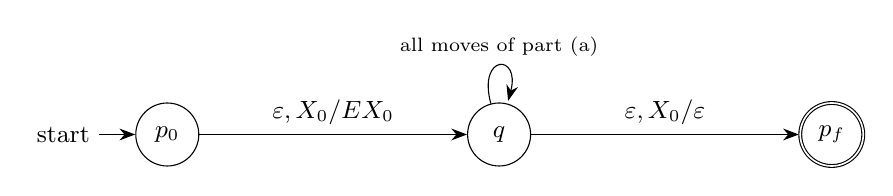
\begin{tikzpicture}[node distance=3.4cm]
\node[state,initial] (p0) {$p_0$};
\node[state,right=of p0] (q) {$q$};
\node[state,accepting,right=of q] (pf) {$p_f$};
\path[->] (p0) edge node {$\eps,X_0/EX_0$} (q) (q) edge node {$\eps,X_0/\eps$} (pf)
 (q) edge[loop above] node[font=\scriptsize] {all moves of part (a)} ();
\end{tikzpicture}
\end{center}
\ansh{Why it works.} If $(q,w,E)\vdash^*(q,\eps,\eps)$ in $P_N$, then in $P_F$:
$(p_0,w,X_0)\vdash(q,w,EX_0)\vdash^*(q,\eps,X_0)\vdash(p_f,\eps,\eps)$ (the same moves with $X_0$ untouched underneath). Conversely $P_F$ can
reach $p_f$ only by rule 3, i.e.\ only when $X_0$ is on top, which is exactly when the simulated $P_N$ has an empty stack after reading the
same input. Hence $L(P_F)=N(P_N)=L(G)$. Example: $(p_0,a,X_0)\vdash(q,a,EX_0)\vdash(q,a,TX_0)\vdash(q,a,FX_0)\vdash(q,a,IX_0)\vdash(q,a,aX_0)
\vdash(q,\eps,X_0)\vdash(p_f,\eps,\eps)$ --- accept.
\end{qa}

\section{Question 3 --- Grammars and the Chomsky hierarchy}\markboth{Q3 Chomsky hierarchy}{}
\begin{qa}{3(a)}{8 marks}
Explain why context-free grammars (CFGs) are called ``context-free''. Define context-sensitive and unrestricted grammars.
\tcblower
\ansh{Why ``context-free''.} Every production of a CFG has a single variable on the left: $A\to\gamma$. Whenever $A$ appears in a sentential
form, it may be replaced by $\gamma$ \emph{regardless of the symbols around it} (its context). E.g.\ with $S\to0S1\mid\eps$, the $S$ in $00S11$
is rewritten exactly as the $S$ in $0S1$.\\
\ansh{Context-sensitive grammar (Type 1).} $G=(V,T,P,S)$ whose productions have the form $\alpha A\beta\to\alpha\gamma\beta$ with
$A\in V$, $\alpha,\beta\in(V\cup T)^*$ and $\gamma\ne\eps$: $A$ may be replaced by $\gamma$ only in the context $\alpha\_\beta$. Equivalently,
every production $u\to v$ is non-contracting, $|u|\le|v|$. ($S\to\eps$ is allowed if $S$ does not appear on any right side.)
Example for $\{a^nb^nc^n\mid n\ge1\}$: $S\to aSBC\mid aBC$, $CB\to BC$, $aB\to ab$, $bB\to bb$, $bC\to bc$, $cC\to cc$.\\
\ansh{Unrestricted grammar (Type 0).} $G=(V,T,P,S)$ with productions $u\to v$ where $u\in(V\cup T)^*V(V\cup T)^*$ (at least one variable)
and $v\in(V\cup T)^*$ is arbitrary, possibly shorter or empty. These generate exactly the recursively enumerable languages.
\end{qa}

\begin{qa}{3(b)}{7 marks}
Explain the Chomsky hierarchy, i.e.\ the relationship among regular languages, context-free languages, context-sensitive languages and
recursively enumerable languages.
\tcblower
\begin{center}\small
\begin{tabular}{@{}llll@{}}
\toprule
Type & Grammar (production form) & Language class & Machine\\\midrule
3 & regular: $A\to aB\mid a\mid\eps$ & regular & finite automaton (DFA/NFA)\\
2 & context-free: $A\to\gamma$ & context-free & pushdown automaton\\
1 & context-sensitive: $\alpha A\beta\to\alpha\gamma\beta$, $\gamma\ne\eps$ & context-sensitive & linear-bounded automaton\\
0 & unrestricted: $u\to v$ & recursively enumerable & Turing machine\\\bottomrule
\end{tabular}
\end{center}
\begin{center}
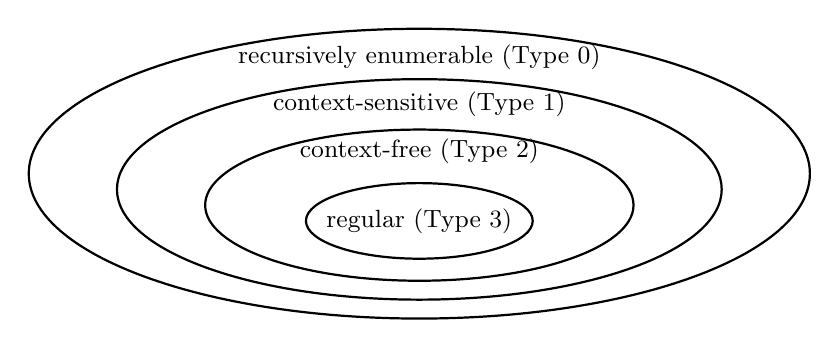
\begin{tikzpicture}[scale=0.8,every node/.style={font=\small}]
\draw[thick] (0,0) ellipse (6.2 and 2.3); \node at (0,1.85) {recursively enumerable (Type 0)};
\draw[thick] (0,-0.25) ellipse (4.8 and 1.75); \node at (0,1.1) {context-sensitive (Type 1)};
\draw[thick] (0,-0.5) ellipse (3.4 and 1.2); \node at (0,0.35) {context-free (Type 2)};
\draw[thick] (0,-0.75) ellipse (1.8 and 0.6); \node at (0,-0.75) {regular (Type 3)};
\end{tikzpicture}
\end{center}
\ansh{Relationship.} Regular $\subsetneq$ CFL $\subsetneq$ CSL $\subsetneq$ RE. Each class contains the one below because each grammar type
is a special case of the next (a regular rule is context-free; a context-free rule $A\to\gamma$ with $\gamma\ne\eps$ is context-sensitive with
empty context; every grammar is unrestricted). Each inclusion is proper:
\begin{itemize}
\item $\{0^n1^n\mid n\ge0\}$ is context-free ($S\to0S1\mid\eps$) but not regular (pumping lemma);
\item $\{a^nb^nc^n\mid n\ge1\}$ is context-sensitive (grammar in 3(a)) but not context-free (CFL pumping lemma);
\item the universal language $\Lu$ (or the halting problem) is RE but not context-sensitive: every CSL is recursive (an LBA has only finitely
many configurations on a given input, so membership can be decided), while $\Lu$ is not recursive.
\end{itemize}
\end{qa}

\section{Question 4 --- TM for 2's complement}\markboth{Q4 TM 2's complement}{}
\begin{qa}{4}{15 marks}
Design a TM that takes as input a number $w$ in binary and computes the 2's complement of the number. The tape initially contains $wc$ where the
leftmost bit is the LSB and $c$ is a separator. Your TM should terminate with the 2's complement of $w$ in binary after the $c$. (You can use multiple
tracks and storage in the state. Recall that two's complement can be formed by copying bits from the left, in this case, until the first 1 and then
by flipping the remaining bits.)
\tcblower
\ansh{Idea.} Process $w$ from the left (LSB first). Keep a flag $f$ in the state: $f=0$ while no 1 has been seen yet, $f=1$ after the first 1.
For each bit $b$: if $f=0$ the output bit is $b$ (copy; a 1 sets $f=1$, so the first 1 itself is copied); if $f=1$ the output bit is $1-b$ (flip).
Mark the processed bit ($0\to X$, $1\to Y$), carry the output bit $o$ and $f$ in the state to the first blank after $c$, write $o$, come back to the
left end, and repeat. When the next unmarked symbol is $c$, restore $X\to0$, $Y\to1$ and halt. The output is written LSB first, like the input.
\[M=(Q,\{0,1,c\},\{0,1,c,X,Y,B\},\delta,s_0,B,\{h\}),\quad Q=\{s_0,s_1,w_{00},w_{11},w_{10},u_{00},u_{11},u_{10},k_0,k_1,\ell,r,h\}\]
($s_f$: find the next bit with flag $f$; $w_{fo}$/$u_{fo}$: carrying new flag $f$ and output bit $o$; $k_f$: return left with flag $f$.)
\begin{center}\small
\begin{tabular}{@{}l|>{\raggedright\arraybackslash}p{13.2cm}@{}}
\toprule
state & $\delta(\text{state},\text{read})=(\text{new state},\text{write},\text{move})$\\\midrule
$s_0$ (no 1 yet) & $X,Y\to$ same, $R$;\quad $0\to(w_{00},X,R)$ \ (copy 0);\quad $1\to(w_{11},Y,R)$ \ (copy the first 1, set flag);\quad $c\to(\ell,c,L)$\\
$s_1$ (1 seen) & $X,Y\to$ same, $R$;\quad $0\to(w_{11},X,R)$ \ (flip: output 1);\quad $1\to(w_{10},Y,R)$ \ (flip: output 0);\quad $c\to(\ell,c,L)$\\
$w_{fo}$ & $0,1\to$ same, $R$;\quad $c\to(u_{fo},c,R)$\\
$u_{fo}$ & $0,1\to$ same, $R$;\quad $B\to(k_f,o,L)$ \ (write the output bit)\\
$k_f$ & $0,1,c,X,Y\to$ same, $L$;\quad $B\to(s_f,B,R)$\\
$\ell$ & $X,Y\to$ same, $L$;\quad $B\to(r,B,R)$\\
$r$ (restore) & $X\to(r,0,R)$;\quad $Y\to(r,1,R)$;\quad $0,1,c\to$ same, $R$;\quad $B\to(h,B,R)$ \ (halt)\\\bottomrule
\end{tabular}
\end{center}
\ansh{Trace on $w=0110$} (LSB first, value $0+2+4=6$), tape after each round:
\[0110c\ \vdash^*\ X110c\mathbf0\ \vdash^*\ XY10c0\mathbf1\ \vdash^*\ XYY0c01\mathbf0\ \vdash^*\ XYYXc010\mathbf1\ \vdash^*\ 0110c0101\ \text{(restore, halt)}.\]
Round 1: $f=0$, copy 0. Round 2: $f=0$, first 1, copy it, $f:=1$. Rounds 3--4: flip $1\to0$, $0\to1$.
Result $0101$ (LSB first) $=2+8=10=2^4-6$: the 4-bit 2's complement of 6. (Checked by program on every input of length 1--7.)
\end{qa}

\section{Question 5 --- Simulations: true or false}\markboth{Q5 Simulations}{}
\begin{qa}{5}{8+7 marks}
Justify whether the following statements are true or false: (i) A deterministic Turing machine can simulate $n$ moves of a conventional computer
in $P(n)$ moves, where $P(n)$ is some polynomial in $n$. (ii) A conventional computer can simulate $n$ moves of a non-deterministic Turing machine
in $P(n)$ moves, where $P(n)$ is some polynomial in $n$.
\tcblower
\ansh{(i) True} --- under the standard assumptions that (a) each instruction makes a word at most one bit longer than its arguments and (b) each
instruction can be done by a multitape TM on $k$-bit words in $O(k^2)$ moves (multiplication is done by shifts and additions).
The TM keeps memory as (address, value) pairs on tape 1, the instruction counter on tape 2 and scratch on tape 3. Let $c$ be the longest word or
address in the program and $d$ the number of words it occupies (constants). After $n$ instructions no word or address is longer than $c+n$ bits
and at most $d+n$ addresses are used, so tape 1 holds at most $2(c+n+1)(d+n)=O(n^2)$ cells. One instruction cycle (find the instruction,
look up its operands, execute, shift over if lengths change, update the counter) scans tape 1 a fixed number of times and works on $O(n)$-bit
words: $O(n^2)$ moves. So $n$ instructions take $O(n^3)$ moves of a multitape TM, and $O((n^3)^2)=O(n^6)$ moves of a one-tape TM (a $k$-tape TM
is simulated by one tape with quadratic slowdown). Both are polynomials.\\[3pt]
\ansh{(ii) False (not known; believed false).} The only known simulation of an NTM $M_N$ is breadth-first search of its computation tree: keep a
queue of IDs, and for the current ID append one copy per possible move. If $M_N$ has at most $m$ choices per move, after $n$ moves there can be
$1+m+m^2+\dots+m^n\le(n+1)m^n$ IDs to examine --- exponential in $n$. A computer is no faster than a DTM up to a polynomial (and vice versa), so a
polynomial-time simulation of $n$ NTM moves would put every NP problem in P, i.e.\ $\P=\NP$, which is not known and is widely believed false.
\end{qa}

\section{Question 6 --- Encoding TMs; $L_d$ is not RE}\markboth{Q6 Diagonalization}{}
\begin{qa}{6(a)}{6 marks}
Briefly explain how a Turing machine (TM) with binary inputs can be encoded using a binary string.
\tcblower
Let $M=(Q,\{0,1\},\Gamma,\delta,q_1,B,F)$. Number everything with positive integers: states $q_1,q_2,\dots,q_r$ with $q_1$ the start state and $q_2$
the only accepting state; tape symbols $X_1=0$, $X_2=1$, $X_3=B$, $X_4,\dots,X_s$ the others; directions $D_1=L$, $D_2=R$.\\
A transition $\delta(q_i,X_j)=(q_k,X_l,D_m)$ is coded as $0^i10^j10^k10^l10^m$ (all of $i,j,k,l,m\ge1$, so a single transition code never
contains $11$). The code of $M$ is the codes of all its transitions separated by $11$: $C_1\,11\,C_2\,11\cdots11\,C_n$.\\
Example: $\delta(q_1,1)=(q_3,0,R)$ is $0\,1\,00\,1\,000\,1\,0\,1\,00=0100100010100$.\\
Binary strings are ordered by length then lexicographically ($w_i$ is the string with $1w_i=i$ in binary: $\eps,0,1,00,\dots$), so ``the $i$-th TM''
$M_i$ is the TM whose code is $w_i$; if $w_i$ is not a valid code, $M_i$ is the TM with no moves ($L(M_i)=\emptyset$).
\end{qa}

\begin{qa}{6(b)}{9 marks}
Prove that the diagonalization language is not recursively enumerable.
\tcblower
\ansh{Definition.} $\Ld=\{w_i\mid w_i\notin L(M_i)\}$: the strings $w$ such that the TM whose code is $w$ does not accept $w$. In the table whose
entry $(i,j)$ is 1 iff $M_i$ accepts $w_j$, $\Ld$ is the complemented diagonal, so it differs from every row $L(M_i)$ at column $i$.\\
\ansh{Theorem.} $\Ld$ is not RE: no TM accepts it.\\
\ansh{Proof.} Suppose, for contradiction, that $\Ld=L(M)$ for some TM $M$. $\Ld$ is a language over $\{0,1\}$, so $M$ has input alphabet $\{0,1\}$
and appears in the enumeration: $M=M_i$ for some $i$ (its code is $w_i$). Ask whether $w_i\in\Ld$.
\begin{itemize}
\item If $w_i\in\Ld$, then $M_i=M$ accepts $w_i$ (because $L(M)=\Ld$). But by the definition of $\Ld$, $w_i\in\Ld$ means $M_i$ does \emph{not} accept $w_i$.
\item If $w_i\notin\Ld$, then $M_i$ does not accept $w_i$. But then, by the definition of $\Ld$, $w_i\in\Ld$.
\end{itemize}
Both cases are impossible, so the assumption is false: no TM accepts $\Ld$, i.e.\ $\Ld$ is not recursively enumerable. $\blacksquare$
\end{qa}

\section{Question 7 --- An RE language that is not recursive}\markboth{Q7 Universal language}{}
\begin{qa}{7}{15 marks}
Provide an example of a language which is recursively enumerable but not recursive. Show that the language you mentioned is recursively
enumerable but not recursive.
\tcblower
\ansh{Example.} The universal language $\Lu=\{(M,w)\mid M$ is a TM with binary input alphabet and $M$ accepts $w\}$ (pairs coded as
$\langle M\rangle111w$).\\
\ansh{$\Lu$ is RE.} The universal TM $U$ accepts it. $U$ has three tapes: tape 1 holds $\langle M\rangle111w$; tape 2 holds $M$'s simulated tape
($X_j$ written as $0^j$, cells separated by 1); tape 3 holds $M$'s state ($q_i$ as $0^i$). $U$ checks that $\langle M\rangle$ is a valid code
(otherwise halts without accepting), copies $w$ to tape 2 in coded form and writes $0$ (state $q_1$) on tape 3. To simulate one move it searches
tape 1 for a transition $0^i10^j10^k10^l10^m$ whose $0^i$ equals tape 3 and $0^j$ equals the scanned symbol on tape 2; it changes tape 3 to $0^k$,
replaces $0^j$ by $0^l$ on tape 2 (shifting over if needed) and moves the tape-2 head to the neighbouring cell on the left ($m=1$) or right ($m=2$).
If no transition matches, $M$ halts and so does $U$; if $M$ enters its accepting state $q_2$, $U$ accepts. So $L(U)=\Lu$, and $\Lu$ is RE.\\
\ansh{Lemma (complement).} If $L$ is recursive then $\overline L$ is recursive: take a TM that always halts for $L$, make its accepting states
non-accepting, and send every halting non-accepting configuration to a new accepting state; it still always halts and accepts exactly $\overline L$.\\
\ansh{$\Lu$ is not recursive.} Suppose $\Lu$ were recursive. By the lemma $\overline{\Lu}$ is recursive, accepted by a TM $M$ that always halts.
Build $M'$: on input $w$, rewrite the tape as $w111w$ and run $M$. If $w=w_i$, the pair is $(M_i,w_i)$, and $M$ accepts it iff $M_i$ does
\emph{not} accept $w_i$, i.e.\ iff $w_i\in\Ld$. So $L(M')=\Ld$. But $\Ld$ is not RE (Question 6(b)), so $M'$ cannot exist --- a contradiction.
Hence $\Lu$ is RE but not recursive. $\blacksquare$\\
(The halting problem $H=\{(M,w)\mid M$ halts on $w\}$ is another example: RE by simulation, and a decider for $H$ would decide $\Lu$.)
\end{qa}

\section{Question 8 --- Cook's theorem and $\P=\NP$}\markboth{Q8 Cook's theorem}{}
\begin{qa}{8(a)}{8 marks}
State Cook's theorem. Explain how Cook's theorem shows that all problems in NP are reducible to the satisfiability problem.
\tcblower
\ansh{Cook's theorem.} SAT (is a given Boolean formula satisfiable?) is NP-complete.\\
\ansh{SAT $\in\NP$.} Guess a truth assignment and evaluate the formula in polynomial time.\\
\ansh{Every $L\in\NP$ reduces to SAT.} Let $L=L(M)$ for a single-tape NTM $M$ that makes at most $p(n)$ moves on every branch for inputs of length
$n$. If $M$ accepts $w$, there are IDs $\alpha_0\vdash\alpha_1\vdash\dots\vdash\alpha_k$, $k\le p(n)$, with $\alpha_0$ initial and $\alpha_k$ accepting; only
cells $0..p(n)$ are used. From $M$ and $w$ we write a formula $F(M,w)$ whose satisfying assignments describe exactly the accepting branches.
Variables ($0\le i,j\le p(n)$): $s(q,j)$ --- state $q$ at step $j$; $l_{ij}$ --- head on cell $i$ at step $j$; $c(i,j,t)$ --- cell $i$ holds $t$ at step $j$;
$u(i,j)$ --- cell $i$ unchanged from step $j$ to $j+1$. Seven rule families:
\begin{enumerate}
\item exactly one state per step: $\bigvee_q s(q,j)$ and $s(q,j)\to\bigwedge_{\hat q\ne q}\neg s(\hat q,j)$;
\item exactly one head position per step; \quad 3.\ exactly one symbol in every cell at every step;
\item[4.] an unchanged cell keeps its symbol: $c(i,j,t)\wedge u(i,j)\to c(i,j+1,t)$;
\item[5.] each step follows $\delta$: for $\delta(q,t)=\{(q_1,t_1,d_1),\dots,(q_m,t_m,d_m)\}$,
$[s(q,j)\wedge l_{ij}\wedge c(i,j,t)]\to\bigwedge_{k\ne i}u(k,j)\wedge\bigvee_r\big(s(q_r,j{+}1)\wedge l_{\phi(r)(j+1)}\wedge c(i,j{+}1,t_r)\big)$;
\item[6.] step 0 is the initial ID $q_0\,w\,B^{p(n)+1-n}$; \quad 7.\ the state at step $p(n)$ is accepting: $s(q_a,p(n))$.
\end{enumerate}
$F(M,w)$ is the AND of all of these. An accepting branch gives a satisfying assignment; conversely a satisfying assignment is, step by step, a
legal accepting computation (the $\vee$ in rule 5 chooses the branch). The formula is written directly from $M$ and $w$; the largest family
(rule 5) has size $O(|Q||\Gamma|p(n)^3)$, a polynomial. So $w\in L\iff F(M,w)\in$ SAT, computed in polynomial time: every problem in NP
reduces to SAT, and SAT is NP-complete.
\end{qa}

\begin{qa}{8(b)}{7 marks}
Explain why finding a polynomial time algorithm for an NP-complete problem implies $\P=\NP$.
\tcblower
$L$ is NP-complete if (1) $L\in\NP$ and (2) every $A\in\NP$ reduces to $L$ in polynomial time. Suppose an NP-complete $L$ has a deterministic
algorithm running in time $q(m)$. Take any $A\in\NP$ and its reduction $f$ to $L$, computable in time $p(n)$, with $x\in A\iff f(x)\in L$.
Since a TM writes at most one symbol per move, $|f(x)|\le p(n)$. To decide $A$: compute $f(x)$ ($p(n)$ steps), then run $L$'s algorithm on it
($q(p(n))$ steps). The total $p(n)+q(p(n))$ is a polynomial, so $A\in\P$. Hence $\NP\subseteq\P$; together with $\P\subseteq\NP$ (a DTM is an NTM
that never has a choice) this gives $\P=\NP$.
\end{qa}

\section{Question 9 --- PSPACE and Savitch's theorem}\markboth{Q9 PSPACE}{}
\begin{qa}{9(a)}{6 marks}
Define the classes of problems PSPACE and NPSPACE. Explain why the problem class P must be a subset of PSPACE.
\tcblower
\ansh{Definitions.} The space complexity $f(n)$ of a TM (all of whose branches halt) is the maximum number of tape cells it scans on any input of
length $n$ (on any branch, for an NTM).
$\PS=\{L\mid L$ is decided by a deterministic TM in polynomial space$\}$;
$\NPS=\{L\mid L$ is decided by a nondeterministic TM in polynomial space$\}$.\\
\ansh{$\P\subseteq\PS$.} If $L\in\P$, a DTM decides $L$ in at most $T(n)$ moves for a polynomial $T$. In each move the head moves to at most one
new cell, so the machine can visit at most $T(n)+1$ cells. That is a polynomial amount of space, so $L\in\PS$. (The same argument gives
$\NP\subseteq\NPS$.)
\end{qa}

\begin{qa}{9(b)}{9 marks}
Explain how Savitch's theorem proves that $\PS=\NPS$.
\tcblower
\ansh{Savitch's theorem.} For $f(n)\ge n$, $\mathrm{NSPACE}(f(n))\subseteq\mathrm{SPACE}(f^2(n))$.\\
\ansh{$\PS\subseteq\NPS$} is immediate: every DTM is an NTM.\\
\ansh{$\NPS\subseteq\PS$.} Let $N$ be an NTM using $f(n)$ space (polynomial). Trying the branches one by one could need exponential space, because a
branch may run $c^{O(f(n))}$ steps and all its choices would have to be recorded. Instead, a DTM solves the more general reachability question
\[\textsc{reach}(I,J,m):\ \text{``can $N$ go from ID $I$ to ID $J$ in at most $m$ moves?''}\]
If $m=1$, check directly whether $I=J$ or $I\vdash J$. Otherwise try every ID $K$ of size $\le f(n)$ in turn and test $\textsc{reach}(I,K,m/2)$
and then $\textsc{reach}(K,J,m/2)$; answer yes if both hold for some $K$. The two recursive calls run one after the other, so at any time the stack
holds one frame per level: $(I,J,m)$, $(I_2,J_2,m/2)$, $(I_3,J_3,m/4)$, \dots --- at most $\log_2m$ frames.\\
\ansh{Space bound.} With $s$ states and $t$ tape symbols, $N$ has at most $s\,f(n)\,t^{f(n)}$ IDs using $f(n)$ cells, so if it accepts it does so
within $m=c^{1+f(n)}$ moves ($c=s+t$). The DTM calls $\textsc{reach}(I_0,J,c^{1+f(n)})$ for the initial ID $I_0$ and every accepting ID $J$. There are
$\log_2c^{1+f(n)}=O(f(n))$ frames, and each frame holds two IDs ($1+f(n)$ cells each) and $m$ in binary ($O(f(n))$ cells), i.e.\ $O(f(n))$ space.
Total: $O(f^2(n))$ space --- a polynomial if $f$ is. So every language in NPSPACE is in PSPACE, and $\PS=\NPS$.
\end{qa}

% ======================================================================= SECTION B
\clearpage
\section*{Section B}\addcontentsline{toc}{section}{Section B}

\section{Question 10 --- Halting problem, DFA, CFG (compulsory)}\markboth{Q10}{}
\begin{qa}{10(a)}{10 marks}
Define the halting problem. Consider the C code below (\texttt{fib(-1)} is called from \texttt{main}). This code will recurse infinitely. But an
LLM chatbot is likely to correctly point out the issue. Does that mean the LLM has solved the halting problem? Why/why not?
\tcblower
\ansh{Halting problem.} $HALT=\{\langle M,w\rangle\mid M$ is a TM (program) that halts on input $w\}$. The problem asks for \emph{one} algorithm that,
for \emph{every} program--input pair, always terminates and answers correctly whether the program halts. Turing proved no such algorithm exists:
$HALT$ is recursively enumerable but undecidable.\\
\ansh{The code.} \texttt{fib(-1)} fails both base cases ($n\ne1,2$) and calls \texttt{fib(-2)}, \texttt{fib(-3)}, \dots; $n$ only decreases, so the
base case is never reached. (On a real machine it ends with a stack overflow, i.e.\ a crash --- not a normal return.)\\
\ansh{No, the LLM has not solved the halting problem.}
\begin{enumerate}
\item \emph{One instance is not the problem.} Undecidability says no algorithm is correct on \emph{all} inputs. Many individual programs are easy
to analyse (this one has an obvious decreasing recursion with unreachable base case); a human, a compiler warning or a static analyser can spot it
too. Deciding special cases has always been possible.
\item \emph{An LLM is not a guaranteed decider.} It is a heuristic pattern matcher: it gives an answer for every program, but nothing guarantees the
answer is right, and on hard programs (e.g.\ one that halts iff an open conjecture such as Goldbach's is false) it can only guess.
\item \emph{Diagonalisation still applies.} If some program $D$ (an LLM is just a program) always answered correctly, build $Q$: ``on input
$\langle P\rangle$, ask $D$ whether $P$ halts on $\langle P\rangle$; if yes, loop forever; if no, halt.'' Running $Q$ on $\langle Q\rangle$: if $D$
says $Q$ halts, $Q$ loops; if $D$ says it loops, $Q$ halts. $D$ is wrong on $\langle Q,\langle Q\rangle\rangle$. So every LLM fails on some input.
\end{enumerate}
Hence correctly diagnosing this program shows only that this instance is easy, not that the halting problem is decidable.
\end{qa}

\begin{qa}{10(b)}{12 marks}
Design a DFA for the language $L=\{w\in\{0,1\}^*\ :\ |w|\ge3$ and the 3rd symbol from the right is $0\}$. Showing only the state diagram would suffice.
\tcblower
\ansh{Design idea.} Whether $w\in L$ depends only on the last three symbols, so each state remembers the last three symbols read: state $xyz$
($x$ = third from the right). Reading $b$ moves $xyz\to yzb$. Accept iff $x=0$. Strings shorter than 3 must be rejected; this is achieved by
starting in state $111$ (as if the input were padded on the left with 1s, which never makes the third symbol from the right 0).
Start $111$; accepting states $000,001,010,011$. Eight states (and 8 are necessary: any two different last-three-symbol histories are
distinguished by a suffix of length $\le2$).
\begin{center}
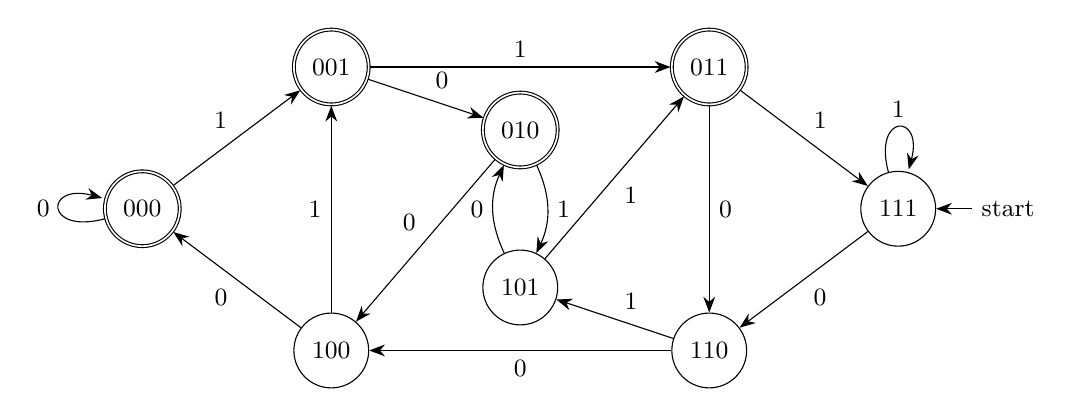
\begin{tikzpicture}[node distance=2cm,every state/.style={minimum size=0.95cm,inner sep=0pt,font=\small}]
\node[state,accepting] (000) at (0,0) {000};
\node[state,accepting] (001) at (2.4,1.8) {001};
\node[state] (100) at (2.4,-1.8) {100};
\node[state,accepting] (010) at (4.8,1.0) {010};
\node[state] (101) at (4.8,-1.0) {101};
\node[state,accepting] (011) at (7.2,1.8) {011};
\node[state] (110) at (7.2,-1.8) {110};
\node[state,initial right] (111) at (9.6,0) {111};
\path[->]
 (000) edge[loop left] node {0} () (000) edge node {1} (001)
 (001) edge node {0} (010) (001) edge node {1} (011)
 (010) edge node[swap] {0} (100) (010) edge[bend left=25] node {1} (101)
 (011) edge node {0} (110) (011) edge node {1} (111)
 (100) edge node {0} (000) (100) edge node {1} (001)
 (101) edge[bend left=25] node {0} (010) (101) edge node[swap] {1} (011)
 (110) edge node {0} (100) (110) edge node[swap] {1} (101)
 (111) edge[loop above] node {1} () (111) edge node {0} (110);
\end{tikzpicture}
\end{center}
\ansh{Check.} $0$: $111\to110$ reject (length 1). $000$: $111\to110\to100\to000$ accept. $1011$: $111\to111\to110\to101\to011$ accept (third from
right is 0). $0100$: $\to110\to101\to010\to100$ reject (third from right is 1). (Checked by program on all strings up to length 12.)
\end{qa}

\begin{qa}{10(c)}{13 marks}
Construct a context-free grammar for the language $L=\{a^nb^mc^n\mid n,m\ge1\}$. Show the parse tree for the string $aabbbcc$ according to your
constructed grammar.
\tcblower
\ansh{Design idea.} The $a$'s and $c$'s are matched from the outside in, so $S$ wraps one $a$ and one $c$ around the middle each time
($S\to aSc$); the innermost wrap ($S\to aBc$) guarantees $n\ge1$ and starts the middle, which is any non-empty block of $b$'s ($B\to bB\mid b$,
$m\ge1$).
\[G=(\{S,B\},\{a,b,c\},P,S),\qquad S\to aSc\mid aBc,\qquad B\to bB\mid b.\]
Every derivation is $S\Rightarrow^*a^{n-1}Sc^{n-1}\Rightarrow a^nBc^n\Rightarrow^*a^nb^mc^n$ with $n,m\ge1$, and every such string is derived this way,
so $L(G)=L$.\\
\ansh{Derivation of $aabbbcc$} ($n=2$, $m=3$): $S\Rightarrow aSc\Rightarrow aaBcc\Rightarrow aabBcc\Rightarrow aabbBcc\Rightarrow aabbbcc$.\\
\ansh{Parse tree.}
\begin{center}
\begin{tikzpicture}[level distance=0.95cm,every node/.style={font=\small},
  level 1/.style={sibling distance=1.6cm},level 2/.style={sibling distance=1.3cm},level 3/.style={sibling distance=1.0cm},
  level 4/.style={sibling distance=0.9cm}]
\node {$S$}
  child {node {$a$}}
  child {node {$S$}
    child {node {$a$}}
    child {node {$B$}
      child {node {$b$}}
      child {node {$B$}
        child {node {$b$}}
        child {node {$B$} child {node {$b$}}}}}
    child {node {$c$}}}
  child {node {$c$}};
\end{tikzpicture}
\end{center}
The yield read left to right is $a\,a\,b\,b\,b\,c\,c$.
\end{qa}

\section{Question 11 --- Pumping lemma; NFA}\markboth{Q11}{}
\begin{qa}{11(a)}{15 marks}
State the pumping lemma for regular languages. Why can the pumping lemma not be used for proving a language is regular? Using the pumping lemma,
prove that $L=\{a^{n^2}\mid n\ge0\}$ is not regular.
\tcblower
\ansh{Pumping lemma.} If $A$ is a regular language, then there is a number $p$ (the pumping length) such that every string $s\in A$ with
$|s|\ge p$ can be divided into three pieces, $s=xyz$, satisfying: (1) $xy^iz\in A$ for every $i\ge0$; (2) $|y|>0$; (3) $|xy|\le p$.\\
\ansh{Why it cannot prove regularity.} The lemma is a one-way implication: regular $\Rightarrow$ pumpable. We use its contrapositive
(not pumpable $\Rightarrow$ not regular). The converse is false --- some non-regular languages satisfy the pumping property, e.g.\
$F=\{a^ib^jc^k\mid i,j,k\ge0,\ i=1\Rightarrow j=k\}$ is not regular, yet every string of length $\ge2$ in $F$ can be pumped. So showing that strings
pump proves nothing; regularity must be shown by a DFA/NFA, a regular expression or closure properties.\\
\ansh{Proof that $L=\{a^{n^2}\}$ is not regular.} Assume, for contradiction, that $L$ is regular, and let $p\ge1$ be its pumping length.
Choose $s=a^{p^2}$; $s\in L$ and $|s|=p^2\ge p$. Let $s=xyz$ be any division with $|y|>0$ and $|xy|\le p$. Since $s$ contains only $a$'s,
$y=a^k$ with $1\le k\le|xy|\le p$. Take $i=2$: $|xy^2z|=p^2+k$, and
\[p^2\ <\ p^2+k\ \le\ p^2+p\ <\ p^2+2p+1=(p+1)^2 .\]
So $p^2+k$ lies strictly between two consecutive perfect squares and is not a perfect square; hence $xy^2z\notin L$. This contradicts the
pumping lemma. Therefore $L$ is not regular. $\blacksquare$
\end{qa}

\begin{qa}{11(b)}{20 marks}
Construct an NFA for $L=\{w\mid w$ contains an even number of 0s, or contains exactly two 1s$\}$ where $\Sigma=\{0,1\}$. Describe your design formally.
Show the state diagram. Show the computation tree for the string $00101$.
\tcblower
\ansh{Design idea.} $L=L_1\cup L_2$ with $L_1$ = even number of 0s and $L_2$ = exactly two 1s. Build a small DFA for each and join them with the
union construction: a new start state $s$ with $\eps$-moves to both start states, so the NFA guesses which condition holds.
\begin{itemize}
\item $L_1$: states $e$ (even number of 0s so far, accepting) and $o$ (odd); a 0 switches $e\leftrightarrow o$, a 1 changes nothing.
\item $L_2$: states $c_0,c_1,c_2$ (number of 1s so far); a 1 moves $c_0\to c_1\to c_2$, a 0 changes nothing; $c_2$ accepting and has
\emph{no} move on 1 (a third 1 kills this branch).
\end{itemize}
\ansh{Formal description.} $N=(Q,\Sigma,\delta,s,F)$ with $Q=\{s,e,o,c_0,c_1,c_2\}$, $\Sigma=\{0,1\}$, start $s$, $F=\{e,c_2\}$ and
\begin{center}\small
\begin{tabular}{c|ccc}
$\delta$ & $0$ & $1$ & $\eps$\\\hline
$\to s$ & $\emptyset$ & $\emptyset$ & $\{e,c_0\}$\\
$*e$ & $\{o\}$ & $\{e\}$ & $\emptyset$\\
$o$ & $\{e\}$ & $\{o\}$ & $\emptyset$\\
$c_0$ & $\{c_0\}$ & $\{c_1\}$ & $\emptyset$\\
$c_1$ & $\{c_1\}$ & $\{c_2\}$ & $\emptyset$\\
$*c_2$ & $\{c_2\}$ & $\emptyset$ & $\emptyset$
\end{tabular}
\end{center}
\begin{center}
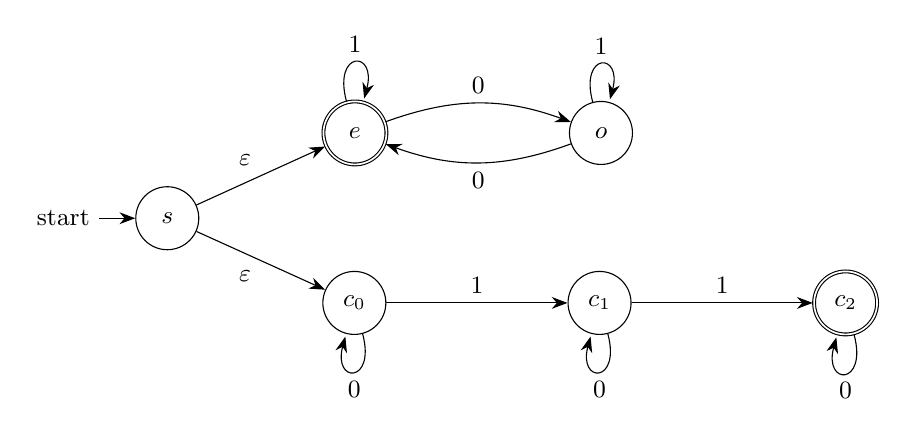
\begin{tikzpicture}[node distance=2.3cm]
\node[state,initial] (s) {$s$};
\node[state,accepting,above right=0.5cm and 1.8cm of s] (e) {$e$};
\node[state,right=of e] (o) {$o$};
\node[state,below right=0.5cm and 1.8cm of s] (c0) {$c_0$};
\node[state,right=of c0] (c1) {$c_1$};
\node[state,accepting,right=of c1] (c2) {$c_2$};
\path[->] (s) edge node {$\eps$} (e) (s) edge node[swap] {$\eps$} (c0)
 (e) edge[bend left=20] node {0} (o) (o) edge[bend left=20] node {0} (e)
 (e) edge[loop above] node {1} () (o) edge[loop above] node {1} ()
 (c0) edge node {1} (c1) (c1) edge node {1} (c2)
 (c0) edge[loop below] node {0} () (c1) edge[loop below] node {0} () (c2) edge[loop below] node {0} ();
\end{tikzpicture}
\end{center}
\ansh{Computation tree for $00101$.} The $\eps$-move splits the computation into two branches at the start; each branch is then deterministic.
\begin{center}
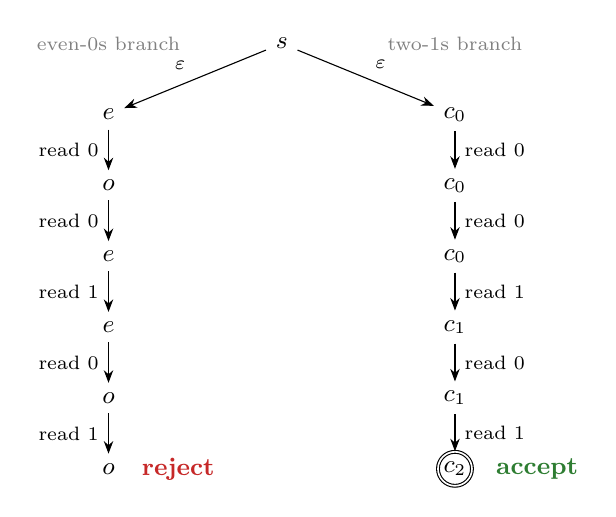
\begin{tikzpicture}[every node/.style={font=\small},>={Stealth[length=1.6mm]}]
\node (s) at (0,0) {$s$};
\foreach \n/\x in {L/-2.2,R/2.2} {}
\node (L0) at (-2.2,-0.9) {$e$};
\node (L1) at (-2.2,-1.8) {$o$}; \node (L2) at (-2.2,-2.7) {$e$}; \node (L3) at (-2.2,-3.6) {$e$};
\node (L4) at (-2.2,-4.5) {$o$}; \node (L5) at (-2.2,-5.4) {$o$}; \node[anchor=west,font=\small\bfseries,color=trapborder] at (-1.9,-5.4) {reject};
\node (R0) at (2.2,-0.9) {$c_0$};
\node (R1) at (2.2,-1.8) {$c_0$}; \node (R2) at (2.2,-2.7) {$c_0$}; \node (R3) at (2.2,-3.6) {$c_1$};
\node (R4) at (2.2,-4.5) {$c_1$}; \node[draw,circle,double,inner sep=1pt] (R5) at (2.2,-5.4) {$c_2$}; \node[anchor=west,font=\small\bfseries,color=exborder] at (2.6,-5.4) {accept};
\draw[->] (s) -- node[above left,font=\scriptsize] {$\eps$} (L0);
\draw[->] (s) -- node[above right,font=\scriptsize] {$\eps$} (R0);
\foreach \a/\b/\c in {0/1/0,1/2/0,2/3/1,3/4/0,4/5/1} {
  \draw[->] (L\a) -- node[left,font=\scriptsize] {read \c} (L\b);
  \draw[->] (R\a) -- node[right,font=\scriptsize] {read \c} (R\b);}
\node[font=\scriptsize,color=gray] at (-2.2,0.0) {even-0s branch};
\node[font=\scriptsize,color=gray] at (2.2,0.0) {two-1s branch};
\end{tikzpicture}
\end{center}
$00101$ has three 0s (odd), so the left branch ends in $o$ and rejects; it has exactly two 1s, so the right branch ends in the accepting state
$c_2$. Since one branch accepts, \textbf{$N$ accepts $00101$}. (The NFA was checked by program on all strings up to length 12.)
\end{qa}

\section{Question 12 --- Languages, grammars and ambiguity}\markboth{Q12}{}
\begin{qa}{12(a)}{7 marks}
What is the main difference between language and grammar?
\tcblower
A \textbf{language} is a \emph{set of strings} over an alphabet --- \emph{what} the valid strings are (e.g.\ $\{0^n1^n\mid n\ge0\}$); it may be infinite.
A \textbf{grammar} $G=(V,T,P,S)$ is a \emph{finite set of rules} that generates strings by derivations from the start symbol --- \emph{how} the strings
are produced (e.g.\ $S\to0S1\mid\eps$). The grammar is a finite description of the (possibly infinite) language $L(G)$. One language can have many
grammars (e.g.\ $S\to0S1\mid\eps$ and $S\to0A\mid\eps,\ A\to S1$ give the same language); the grammar also gives structure (parse trees), which the
language alone does not, and properties such as ambiguity belong to the grammar.
\end{qa}

\begin{qa}{12(b)}{10 marks}
Differentiate between: ambiguous derivation, ambiguous grammar and ambiguous language. Give an example of an inherently ambiguous language.
\tcblower
\ansh{Ambiguous derivation (of a string).} A string $w$ is derived ambiguously in $G$ if it has two or more different parse trees --- equivalently,
two or more different leftmost derivations. Example: in $E\to E+E\mid E\times E\mid a$, the string $a+a\times a$ has the trees $a+(a\times a)$
($E\Rightarrow E+E\Rightarrow a+E\Rightarrow a+E\times E\Rightarrow\dots$) and $(a+a)\times a$ ($E\Rightarrow E\times E\Rightarrow E+E\times E\Rightarrow\dots$).\\
\ansh{Ambiguous grammar.} A grammar $G$ is ambiguous if it generates \emph{at least one} string ambiguously. The grammar above is ambiguous; the
grammar $E\to E+T\mid T$, $T\to T\times F\mid F$, $F\to(E)\mid a$ generates the same language unambiguously. So ambiguity of a grammar can sometimes be
removed.\\
\ansh{Ambiguous (inherently ambiguous) language.} A context-free language is inherently ambiguous if \emph{every} grammar for it is ambiguous ---
the ambiguity cannot be removed by rewriting the grammar. This is a property of the language, not of one grammar.\\
\ansh{Example.} $L=\{a^ib^jc^k\mid i=j\text{ or }j=k\}$. A grammar: $S\to S_1C\mid AS_2$, $S_1\to aS_1b\mid\eps$, $C\to cC\mid\eps$,
$A\to aA\mid\eps$, $S_2\to bS_2c\mid\eps$. Every string $a^nb^nc^n$ belongs to both parts and gets two parse trees (e.g.\ $abc$:
$S\Rightarrow S_1C\Rightarrow abC\Rightarrow abc$ and $S\Rightarrow AS_2\Rightarrow aS_2\Rightarrow abc$); every grammar for $L$ must likewise generate
these strings by both mechanisms, so $L$ is inherently ambiguous. (Another: $\{a^nb^nc^md^m\}\cup\{a^nb^mc^md^n\}$.)
\end{qa}

\begin{qa}{12(c)}{18 marks}
Let $\Sigma=\{a,b,c\}$. Give a CFG that generates the language of strings such that $n_a+n_b=n_c$, where $n_a,n_b,n_c$ are the numbers of $a$'s, $b$'s
and $c$'s respectively. Explain your reasoning.
\tcblower
\ansh{Idea.} Call $a$ and $b$ ``plus'' symbols and $c$ a ``minus'' symbol. The condition $n_a+n_b=n_c$ says every $c$ is paired with one $a$ or $b$,
in any order --- exactly like ``equal numbers of 0s and 1s'', where 0 can be either $a$ or $b$. That language has the grammar
$S\to0S1S\mid1S0S\mid\eps$; replace 0 by $a$ or $b$:
\[G:\quad S\to aScS\ \mid\ bScS\ \mid\ cSaS\ \mid\ cSbS\ \mid\ \eps .\]
\ansh{Every generated string satisfies $n_a+n_b=n_c$.} By induction on the length of the derivation: $\eps$ has all counts 0, and each non-empty
rule adds exactly one $a$ or $b$ and exactly one $c$, so the difference $d=(n_a+n_b)-n_c$ stays 0.\\
\ansh{Every string with $n_a+n_b=n_c$ is generated.} Strong induction on $|w|$. If $w=\eps$, use $S\to\eps$. Otherwise suppose $w$ starts with $a$
(the cases $b$ and $c$ are symmetric). For prefixes $u$ of $w$ let $d(u)=(n_a+n_b)(u)-n_c(u)$; $d$ is 1 after the first symbol, 0 at the end, and
changes by $\pm1$ per symbol. Take the first point after the first symbol where $d=0$; the symbol that brought $d$ from 1 to 0 is a $c$. So
$w=a\,x\,c\,y$ with $d(x)=0$ and $d(y)=0$: both $x$ and $y$ satisfy the condition and are shorter than $w$. By the induction hypothesis
$S\Rightarrow^*x$ and $S\Rightarrow^*y$, so $S\Rightarrow aScS\Rightarrow^*axcy=w$. (If $w$ starts with $c$, the first return to $d=0$ is caused by an $a$ or $b$
and we use $cSaS$ or $cSbS$.)\\
\ansh{Example.} $acbc$ ($n_a+n_b=2=n_c$): $S\Rightarrow aScS\Rightarrow acS\Rightarrow acbScS\Rightarrow acbcS\Rightarrow acbc$.
(The grammar was checked by program against the definition on all strings up to length 8.)
\end{qa}

\section{Question 13 --- CFL pumping lemma, reversal, Thompson's construction}\markboth{Q13}{}
\begin{qa}{13(a)}{12 marks}
Using the pumping lemma for CFGs, prove that $L=\{a^nb^mc^nd^m\mid n,m\ge0\}$ is not context-free.
\tcblower
\ansh{Pumping lemma for CFLs.} If $L$ is context-free, there is a number $p$ such that every $w\in L$ with $|w|\ge p$ can be written $w=uvxyz$ with
(1) $uv^ixy^iz\in L$ for all $i\ge0$, (2) $|vy|>0$, (3) $|vxy|\le p$.\\
\ansh{Proof.} Assume, for contradiction, that $L$ is context-free, and let $p$ be its pumping length. Choose $w=a^pb^pc^pd^p\in L$
($n=m=p$); $|w|=4p\ge p$. Let $w=uvxyz$ be any division with $|vy|>0$ and $|vxy|\le p$. Since each block has length $p$, the window $vxy$ lies within
at most two \emph{adjacent} blocks ($a$/$b$, $b$/$c$ or $c$/$d$). Pump with $i=2$:
\begin{itemize}
\item If $v$ or $y$ contains two different letters, then $uv^2xy^2z$ has letters out of order (e.g.\ a $b$ before an $a$), so it is not of the form
$a^*b^*c^*d^*$ and not in $L$.
\item Otherwise each of $v$, $y$ lies inside one block, and pumping increases the length of one or two adjacent blocks; since $|vy|>0$ at least one
block grows. If the $a$-block or the $c$-block grows, its partner (the $c$-block or the $a$-block) is not adjacent to it, so it lies outside $vxy$
and is unchanged: $\#a\ne\#c$. Otherwise only the $b$- and/or $d$-blocks change, and a growing $b$-block (or $d$-block) has its non-adjacent partner
unchanged: $\#b\ne\#d$.
\end{itemize}
In every case $uv^2xy^2z\notin L$, contradicting the pumping lemma. Therefore $L$ is not context-free. $\blacksquare$
\end{qa}

\begin{qa}{13(b)}{10 marks}
Formally prove that ``the class of regular languages is closed under reversal''.
\tcblower
\ansh{Claim.} If $A$ is regular then $A^R=\{w^R\mid w\in A\}$ is regular.\\
\ansh{Construction.} Let $M=(Q,\Sigma,\delta,q_0,F)$ be a DFA with $L(M)=A$. Build the NFA $N=(Q\cup\{s\},\Sigma,\delta_R,s,\{q_0\})$, $s\notin Q$, by
reversing every arrow, starting from all old accepting states and accepting in the old start state:
\[\delta_R(s,\eps)=F,\qquad \delta_R(q,a)=\{p\in Q\mid \delta(p,a)=q\}\ \ (q\in Q,\ a\in\Sigma),\qquad \delta_R(s,a)=\emptyset,\ \ \delta_R(q,\eps)=\emptyset .\]
\ansh{Lemma.} For all $p,q\in Q$ and $w\in\Sigma^*$: $\hat\delta(p,w)=q$ in $M$ $\iff$ $N$ can go from $q$ to $p$ reading $w^R$ (without
$\eps$-moves).\\
\emph{Proof by induction on $|w|$.} $w=\eps$: both sides say $p=q$. $w=ua$: $\hat\delta(p,ua)=q$ iff there is $r$ with $\hat\delta(p,u)=r$ and
$\delta(r,a)=q$. By the definition of $\delta_R$, $\delta(r,a)=q$ iff $r\in\delta_R(q,a)$, i.e.\ $N$ goes from $q$ to $r$ reading $a$; by the
induction hypothesis $\hat\delta(p,u)=r$ iff $N$ goes from $r$ to $p$ reading $u^R$. Together: $N$ goes from $q$ to $p$ reading $a\,u^R=(ua)^R$. \hfill$\square$\\
\ansh{Correctness.}
$w\in A\iff\hat\delta(q_0,w)=f$ for some $f\in F\iff$ (lemma) $N$ goes from some $f\in F$ to $q_0$ reading $w^R\iff$ $N$ accepts $w^R$ (it starts
in $s$, takes $s\xrightarrow{\eps}f$, and $q_0$ is its only accepting state). Hence $L(N)=A^R$. $N$ is an NFA, and NFAs recognise exactly the
regular languages, so $A^R$ is regular. $\blacksquare$\\
(Alternative: by induction on a regular expression, $a^R=a$, $\eps^R=\eps$, $\emptyset^R=\emptyset$, $(R_1\cup R_2)^R=R_1^R\cup R_2^R$,
$(R_1R_2)^R=R_2^RR_1^R$, $(R^*)^R=(R^R)^*$, so every regular expression has a reversed regular expression.)
\end{qa}

\begin{qa}{13(c)}{13 marks}
Convert the regular expression $R=(ab^*c\cup ac)^*$ to an NFA using Thompson's construction.
\tcblower
\ansh{Build bottom-up,} one NFA per sub-expression, using the basic NFAs for single symbols and the union, concatenation and star constructions.
\begin{enumerate}
\item $a$: $n_1\xrightarrow{a}n_2$.\quad $b$: $n_4\xrightarrow{b}n_5$.\quad $c$: $n_6\xrightarrow{c}n_7$.
\item $b^*$: new accepting start $n_3$, $n_3\xrightarrow{\eps}n_4$, and $n_5\xrightarrow{\eps}n_4$ (repeat). Accepting: $n_3,n_5$.
\item $ab^*c$: concatenate: $n_2\xrightarrow{\eps}n_3$, and from the accepting states of $b^*$: $n_3\xrightarrow{\eps}n_6$, $n_5\xrightarrow{\eps}n_6$.
Start $n_1$, accept $n_7$.
\item $ac$: $n_8\xrightarrow{a}n_9\xrightarrow{\eps}n_{10}\xrightarrow{c}n_{11}$. Start $n_8$, accept $n_{11}$.
\item $ab^*c\cup ac$: new start $n_0$ with $n_0\xrightarrow{\eps}n_1$ and $n_0\xrightarrow{\eps}n_8$. Accepting $n_7,n_{11}$.
\item $(ab^*c\cup ac)^*$: new accepting start $S$ with $S\xrightarrow{\eps}n_0$, and $n_7\xrightarrow{\eps}n_0$, $n_{11}\xrightarrow{\eps}n_0$.
Accepting states: $S,n_7,n_{11}$.
\end{enumerate}
\begin{center}
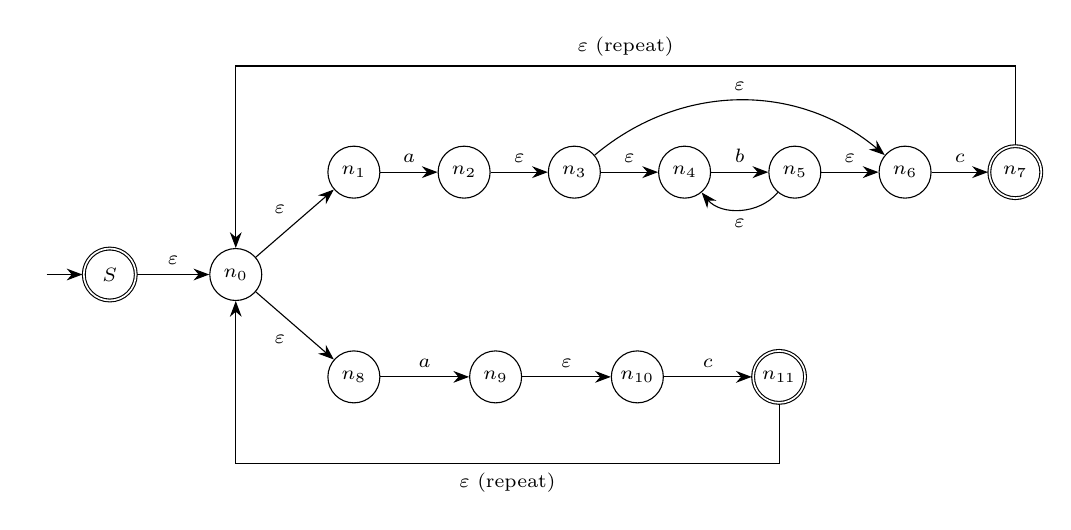
\begin{tikzpicture}[every state/.style={minimum size=0.66cm,inner sep=0pt,font=\scriptsize},every edge/.append style={font=\scriptsize}]
\node[state,initial,initial text=,accepting] (S) at (0,0) {$S$};
\node[state] (n0) at (1.6,0) {$n_0$};
\node[state] (n1) at (3.1,1.3) {$n_1$};
\node[state] (n2) at (4.5,1.3) {$n_2$};
\node[state] (n3) at (5.9,1.3) {$n_3$};
\node[state] (n4) at (7.3,1.3) {$n_4$};
\node[state] (n5) at (8.7,1.3) {$n_5$};
\node[state] (n6) at (10.1,1.3) {$n_6$};
\node[state,accepting] (n7) at (11.5,1.3) {$n_7$};
\node[state] (n8) at (3.1,-1.3) {$n_8$};
\node[state] (n9) at (4.9,-1.3) {$n_9$};
\node[state] (n10) at (6.7,-1.3) {$n_{10}$};
\node[state,accepting] (n11) at (8.5,-1.3) {$n_{11}$};
\path[->] (S) edge node {$\eps$} (n0)
 (n0) edge node {$\eps$} (n1) (n0) edge node[swap] {$\eps$} (n8)
 (n1) edge node {$a$} (n2) (n2) edge node {$\eps$} (n3) (n3) edge node {$\eps$} (n4) (n4) edge node {$b$} (n5)
 (n5) edge[bend left=50] node {$\eps$} (n4) (n5) edge node {$\eps$} (n6) (n3) edge[bend left=40] node {$\eps$} (n6)
 (n6) edge node {$c$} (n7)
 (n8) edge node {$a$} (n9) (n9) edge node {$\eps$} (n10) (n10) edge node {$c$} (n11);
\draw[->] (n7.north) -- ++(0,1.0) -| node[pos=0.25,above,font=\scriptsize] {$\eps$\ (repeat)} (n0.north);
\draw[->] (n11.south) -- ++(0,-0.75) -| node[pos=0.25,below,font=\scriptsize] {$\eps$\ (repeat)} (n0.south);
\end{tikzpicture}
\end{center}
\ansh{Check.} $\eps$: accepted at $S$. $abbc$: $S\to n_0\to n_1\xrightarrow{a}n_2\to n_3\to n_4\xrightarrow{b}n_5\to n_4\xrightarrow{b}n_5\to n_6\xrightarrow{c}n_7$ accept.
$acac$: through the lower branch twice ($n_{11}\xrightarrow{\eps}n_0$) --- accept. $ab$: never reaches an accepting state --- reject. (The NFA was
compared with $(ab^*c\cup ac)^*$ by program on all strings up to length 10.)
\end{qa}

\end{document}
